% Options for packages loaded elsewhere
\PassOptionsToPackage{unicode}{hyperref}
\PassOptionsToPackage{hyphens}{url}
%
\documentclass[
  letterpaper,
  oneside,
  open=any]{scrbook}

\usepackage{amsmath,amssymb}
\usepackage{iftex}
\ifPDFTeX
  \usepackage[T1]{fontenc}
  \usepackage[utf8]{inputenc}
  \usepackage{textcomp} % provide euro and other symbols
\else % if luatex or xetex
  \usepackage{unicode-math}
  \defaultfontfeatures{Scale=MatchLowercase}
  \defaultfontfeatures[\rmfamily]{Ligatures=TeX,Scale=1}
\fi
\usepackage{lmodern}
\ifPDFTeX\else  
    % xetex/luatex font selection
\fi
% Use upquote if available, for straight quotes in verbatim environments
\IfFileExists{upquote.sty}{\usepackage{upquote}}{}
\IfFileExists{microtype.sty}{% use microtype if available
  \usepackage[]{microtype}
  \UseMicrotypeSet[protrusion]{basicmath} % disable protrusion for tt fonts
}{}
\makeatletter
\@ifundefined{KOMAClassName}{% if non-KOMA class
  \IfFileExists{parskip.sty}{%
    \usepackage{parskip}
  }{% else
    \setlength{\parindent}{0pt}
    \setlength{\parskip}{6pt plus 2pt minus 1pt}}
}{% if KOMA class
  \KOMAoptions{parskip=half}}
\makeatother
\usepackage{xcolor}
\setlength{\emergencystretch}{3em} % prevent overfull lines
\setcounter{secnumdepth}{5}
% Make \paragraph and \subparagraph free-standing
\ifx\paragraph\undefined\else
  \let\oldparagraph\paragraph
  \renewcommand{\paragraph}[1]{\oldparagraph{#1}\mbox{}}
\fi
\ifx\subparagraph\undefined\else
  \let\oldsubparagraph\subparagraph
  \renewcommand{\subparagraph}[1]{\oldsubparagraph{#1}\mbox{}}
\fi

\providecommand{\tightlist}{%
  \setlength{\itemsep}{0pt}\setlength{\parskip}{0pt}}\usepackage{longtable,booktabs,array}
\usepackage{calc} % for calculating minipage widths
% Correct order of tables after \paragraph or \subparagraph
\usepackage{etoolbox}
\makeatletter
\patchcmd\longtable{\par}{\if@noskipsec\mbox{}\fi\par}{}{}
\makeatother
% Allow footnotes in longtable head/foot
\IfFileExists{footnotehyper.sty}{\usepackage{footnotehyper}}{\usepackage{footnote}}
\makesavenoteenv{longtable}
\usepackage{graphicx}
\makeatletter
\def\maxwidth{\ifdim\Gin@nat@width>\linewidth\linewidth\else\Gin@nat@width\fi}
\def\maxheight{\ifdim\Gin@nat@height>\textheight\textheight\else\Gin@nat@height\fi}
\makeatother
% Scale images if necessary, so that they will not overflow the page
% margins by default, and it is still possible to overwrite the defaults
% using explicit options in \includegraphics[width, height, ...]{}
\setkeys{Gin}{width=\maxwidth,height=\maxheight,keepaspectratio}
% Set default figure placement to htbp
\makeatletter
\def\fps@figure{htbp}
\makeatother

\usepackage[default]{opensans}
\fontseries{lc}\selectfont
\definecolor{nmfsblue1}{HTML}{00467f}
\definecolor{nmfsblue2}{HTML}{007eb2}
\makeatletter
\@ifpackageloaded{bookmark}{}{\usepackage{bookmark}}
\makeatother
\makeatletter
\@ifpackageloaded{caption}{}{\usepackage{caption}}
\AtBeginDocument{%
\ifdefined\contentsname
  \renewcommand*\contentsname{Table of contents}
\else
  \newcommand\contentsname{Table of contents}
\fi
\ifdefined\listfigurename
  \renewcommand*\listfigurename{List of Figures}
\else
  \newcommand\listfigurename{List of Figures}
\fi
\ifdefined\listtablename
  \renewcommand*\listtablename{List of Tables}
\else
  \newcommand\listtablename{List of Tables}
\fi
\ifdefined\figurename
  \renewcommand*\figurename{Figure}
\else
  \newcommand\figurename{Figure}
\fi
\ifdefined\tablename
  \renewcommand*\tablename{Table}
\else
  \newcommand\tablename{Table}
\fi
}
\@ifpackageloaded{float}{}{\usepackage{float}}
\floatstyle{ruled}
\@ifundefined{c@chapter}{\newfloat{codelisting}{h}{lop}}{\newfloat{codelisting}{h}{lop}[chapter]}
\floatname{codelisting}{Listing}
\newcommand*\listoflistings{\listof{codelisting}{List of Listings}}
\makeatother
\makeatletter
\makeatother
\makeatletter
\@ifpackageloaded{caption}{}{\usepackage{caption}}
\@ifpackageloaded{subcaption}{}{\usepackage{subcaption}}
\makeatother

\usepackage{hyphenat}
\usepackage{ifthen}
\usepackage{calc}
\usepackage{calculator}

\usepackage{graphicx}
\usepackage{wallpaper}

\usepackage{geometry}

\usepackage{graphicx}
\usepackage{geometry}
\usepackage{afterpage}
\usepackage{tikz}
\usetikzlibrary{calc}
\usetikzlibrary{fadings}
\usepackage[pagecolor=none]{pagecolor}


% Set the titlepage font families







% Set the coverpage font families

\ifLuaTeX
  \usepackage{selnolig}  % disable illegal ligatures
\fi
\usepackage[]{biblatex}
\addbibresource{text/references.bib}
\usepackage{bookmark}

\IfFileExists{xurl.sty}{\usepackage{xurl}}{} % add URL line breaks if available
\urlstyle{same} % disable monospaced font for URLs
\hypersetup{
  pdftitle={Vessel presence in Two Rocks Marine Park assessed using passive acoustic monitoring},
  pdfauthor={Rochelle Gordon; Jessica A. McCordic; Sofie M. Van Parijs},
  hidelinks,
  pdfcreator={LaTeX via pandoc}}

\title{Vessel presence in Two Rocks Marine Park assessed using passive
acoustic monitoring}
\usepackage{etoolbox}
\makeatletter
\providecommand{\subtitle}[1]{% add subtitle to \maketitle
  \apptocmd{\@title}{\par {\large #1 \par}}{}{}
}
\makeatother
\subtitle{Report prepared by NOAA Northeast Fisheries Science Center for
Parks Australia}
\author{Rochelle Gordon \and Jessica A. McCordic \and Sofie M. Van
Parijs}
\date{2023-01-01}

\begin{document}
%%%%% begin titlepage extension code

  \begin{frontmatter}

\begin{titlepage}

%%% TITLE PAGE START

% Set up alignment commands
%Page
\newcommand{\titlepagepagealign}{
\ifthenelse{\equal{left}{right}}{\raggedleft}{}
\ifthenelse{\equal{left}{center}}{\centering}{}
\ifthenelse{\equal{left}{left}}{\raggedright}{}
}
%% Titles
\newcommand{\titlepagetitlealign}{
\ifthenelse{\equal{left}{right}}{\raggedleft}{}
\ifthenelse{\equal{left}{center}}{\centering}{}
\ifthenelse{\equal{left}{left}}{\raggedright}{}
\ifthenelse{\equal{left}{spread}}{\makebox[\linewidth][s]}{}
}


\newcommand{\titleandsubtitle}{
% Title and subtitle
{\fontsize{30}{36.0}\selectfont
\textcolor{nmfsblue1}{\bfseries{\nohyphens{Vessel presence in Two Rocks
Marine Park assessed using passive acoustic monitoring}}}\par
}%

\vspace{\betweentitlesubtitle}
{
{\textit{\nohyphens{Report prepared by NOAA Northeast Fisheries Science
Center for Parks Australia}}}\par
}}
\newcommand{\titlepagetitleblock}{
\titleandsubtitle
}

\newcommand{\authorstyle}[1]{{\fontsize{20}{24.0}\selectfont
#1}}

\newcommand{\affiliationstyle}[1]{{#1}}

\newcommand{\titlepageauthorblock}{
{\authorstyle{\nohyphens{Rochelle
Gordon}{\textsuperscript{1}}\textsuperscript{,}{\textsuperscript{2}},  \nohyphens{Jessica
A. McCordic}{\textsuperscript{1}} and \nohyphens{Sofie M. Van
Parijs}{\textsuperscript{1}}}}}

\newcommand{\titlepageaffiliationblock}{
\hangindent=1em
\hangafter=1
{\affiliationstyle{
{1}.~Northeast Fisheries Science Center,~Protected Species Division,~166
Water StreetWoods Hole, Massachusetts 02543
\par\hangindent=1em\hangafter=1{2}.~Azura Consulting, LLC.


\vspace{1\baselineskip} 
}}
}
\newcommand{\headerstyled}{%
{}
}
\newcommand{\footerstyled}{%
{}
}
\newcommand{\datestyled}{%
{2023-01-01}
}


\newcommand{\titlepageheaderblock}{\headerstyled}

\newcommand{\titlepagefooterblock}{
\footerstyled
}

\newcommand{\titlepagedateblock}{
\datestyled
}

%set up blocks so user can specify order
\newcommand{\titleblock}{\newlength{\betweentitlesubtitle}
\setlength{\betweentitlesubtitle}{1pt}
{\titlepagetitlealign

{\titlepagetitleblock}
}

\vspace{4\baselineskip}
}

\newcommand{\authorblock}{{\titlepageauthorblock}

\vspace{2\baselineskip}
}

\newcommand{\affiliationblock}{{\titlepageaffiliationblock}

\vspace{2\baselineskip}
}

\newcommand{\logoblock}{}

\newcommand{\footerblock}{}

\newcommand{\dateblock}{{\titlepagedateblock}

\vspace{0pt}
}

\newcommand{\headerblock}{}
\newgeometry{top=3in,bottom=1in,right=1in,left=1.75in}
% background image
\newlength{\bgimagesize}
\setlength{\bgimagesize}{0.75\paperwidth}
\LENGTHDIVIDE{\bgimagesize}{\paperwidth}{\theRatio} % from calculator pkg
\ThisULCornerWallPaper{\theRatio}{images/corner-image.png}

\thispagestyle{empty} % no page numbers on titlepages


\newcommand{\vrulecode}{\rule{\vrulewidth}{\textheight}}
\newlength{\vrulewidth}
\setlength{\vrulewidth}{0pt}
\newlength{\B}
\setlength{\B}{\ifdim\vrulewidth > 0pt 0.05\textwidth\else 0pt\fi}
\newlength{\minipagewidth}
\ifthenelse{\equal{left}{left} \OR \equal{left}{right} }
{% True case
\setlength{\minipagewidth}{\textwidth - \vrulewidth - \B - 0.1\textwidth}
}{
\setlength{\minipagewidth}{\textwidth - 2\vrulewidth - 2\B - 0.1\textwidth}
}
\ifthenelse{\equal{left}{left} \OR \equal{left}{leftright}}
{% True case
\raggedleft % needed for the minipage to work
\vrulecode
\hspace{\B}
}{%
\raggedright % else it is right only and width is not 0
}
% [position of box][box height][inner position]{width}
% [s] means stretch out vertically; assuming there is a vfill
\begin{minipage}[b][\textheight][s]{\minipagewidth}
\titlepagepagealign
\headerblock

\titleblock

\authorblock

\affiliationblock

\vfill

\logoblock

\footerblock
\par

\end{minipage}\ifthenelse{\equal{left}{right} \OR \equal{left}{leftright} }{
\hspace{\B}
\vrulecode}{}
\clearpage
\restoregeometry
%%% TITLE PAGE END
\end{titlepage}
\setcounter{page}{1}
\end{frontmatter}

%%%%% end titlepage extension code

\renewcommand*\contentsname{Table of contents}
{
\setcounter{tocdepth}{1}
\tableofcontents
}
\listoffigures
\listoftables
\mainmatter
\bookmarksetup{startatroot}

\chapter*{Citation}\label{citation}
\addcontentsline{toc}{chapter}{Citation}

\markboth{Citation}{Citation}

Gordon, R., McCordic, J. A., VanParjis, S. M., year. AMP Report.
Northeast Fisheries Science Center.

\bookmarksetup{startatroot}

\chapter{Site description and recording
effort}\label{site-description-and-recording-effort}

Two Rocks Marine Park is part of the South-west Regional Management
Network of the Australian Marine Parks system. The selected National
Park Zone (NPZ) (swtwonpz02) represents a relatively shallow coastal
habitat with a bottom type primarily consisting of calcareous sand and
gravel (Lucieer et al.~2017). Recorders were deployed at two sites
within the NPZ---Two Rocks East (TRE) and Two Rocks West (TRW)---to
maximize coverage of the monitoring area (Table 1, Fig. 1).

\textbf{Table 1:} Summary of recording effort
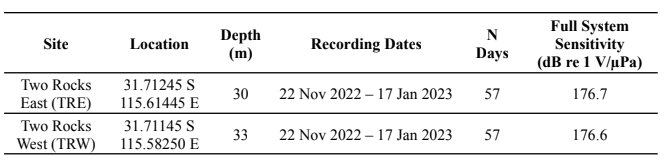
\includegraphics{images/Table.1.PNG}

\begin{figure}[H]

{\centering 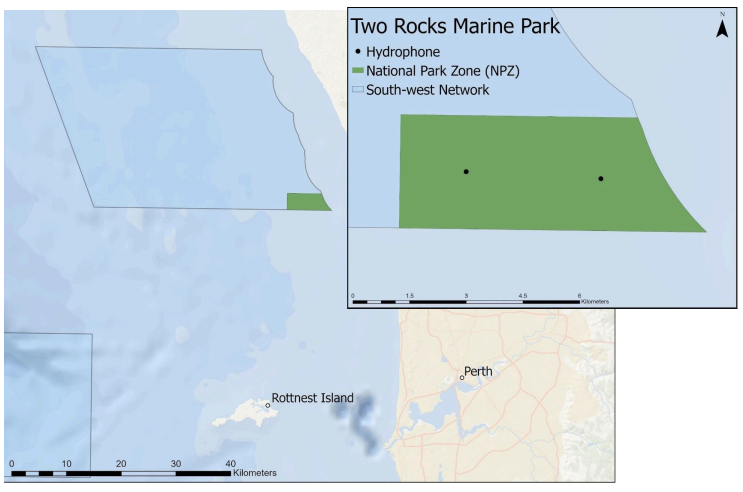
\includegraphics{images/Fig.1.PNG}

}

\caption{\textbf{Figure 1:} Map of Soundtrap deployment sites within Two
Rocks Marine Park. Green shaded region indicates NPZ boundary within
larger marine park}

\end{figure}%

\section{Propagation modeling}\label{propagation-modeling}

The calibration tracks resulted in 156 location selections for TRE and
333 location selections for TRW. After reviewing the peak frequency
measurements and iteratively removing outliers using Matlab's Curve
Fitting tool, 154 points from TRE and 165 points from TRE were used in
the final model of transmission loss.

\section{Detecting unknown vessels}\label{detecting-unknown-vessels}

Using the Ship Detector Remora attached to Triton software (version
1.93.20160524), potential vessel passages were automatically selected
from a long-term spectral average (LTSA) of each deployment. We
conducted a hybrid methodology using the results from the detector with
a manual review of the data at one site to examine whether the detector
performance was sufficient for this project. All vessel detections at
both TRE and TRW were reviewed using spectrograms in Raven Pro 2.0 as
described in the SOP to determine start and end times. For TRE, after
running the detector, we manually reviewed the LTSA calculated in Triton
to look for any vessel signatures that may have been missed by the
detector. Potential vessels found during this step were compared against
the start and end times of automated detections to determine if they
were new vessels. Following review of TRE, a subset of the first 19 days
of the TRW deployment (33\% of days) were manually reviewed for vessels
missed by the detector. Precision of the detector was calculated for
both sites following manual review of detected events using the full
deployment length at TRE and the 19-day subset at TRW.

\section{Determining vessel presence within MPA
boundaries}\label{determining-vessel-presence-within-mpa-boundaries}

A subset of suitable vessels was further analyzed to determine the
likelihood of occurring within the NPZ boundaries based on modeled
values of source level for each vessel and transmission loss at each
site. Furthermore, the vessel behavioral categories were simplified from
previous deployments and included two categories: transiting (T) and
maneuvering (M) vessels.

\bookmarksetup{startatroot}

\chapter{Results}\label{results}

\section{Detector Performance}\label{detector-performance}

The vessel detector found a total of 487 events at TRE and 546 events at
TRW. Of the events at TRE, 54 events were correctly identified as
vessels, and 162 were correctly identified as ambient noise. An
additional 9 ambient events were incorrectly identified as vessels, and
262 true ship events were incorrectly classified as ambient noise (Table
2). After manual review of the LTSA, 344 vessels missed by the detector
were added to the analysis for TRE. Including these added vessels as
false negatives, this detector has a recall value of 0.08 and a
precision value of 0.86 (Table 2).

At TRW, the detector correctly classified 60 events as vessels and 195
events as ambient noise. There were 4 false positive events where the
detector incorrectly classified ambient noise as ship events and 287
false negative events where ships were incorrectly classified as ambient
noise. Manual review of the LTSA was completed for the first 19 days of
the deployment, in which 29 additional vessel passages were observed.
The precision of the TRW detector (0.93) was similar to TRE (0.86).

The total number of detected ship events at both sites includes vessel
events under 500 Hz, which are not used in further analysis throughout
this report.

\textbf{Table 2:} Detection matrix for automated ship detector used in
Two Rocks East site. The predicted condition indicates the number of
events the detector identified as either ``ship'' or ``ambient'', and
the true condition indicates the number of events identified by manually
reviewing the detections and the LTSA.
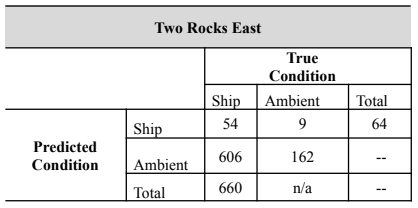
\includegraphics{images/Table.2.PNG}

\section{Overall Patterns of Vessel
Presence}\label{overall-patterns-of-vessel-presence}

After manually reviewing the detections and the LTSA, TRE had a total
vessel count of 660 signatures. For TRW, manual review of detections
resulted in a total of 377 vessel signatures. At both sites, vessel
activity occurred throughout the deployment, although vessels were not
present every day. At TRE, vessels occurred on 56/57 days (98.2\% of
days, mean of 11.7 vessels/day present), and in TRW vessels occurred on
54/57 days (94.7\% of days, mean of 7 vessels/day present).

Both sites showed similarities in duration of individual vessel
signatures, with median values within 5 minutes (TRE = 24.2 minutes; TRW
= 30.3 minutes); however, TRW showed a much greater range of durations,
with the longest continuous vessel signature lasting over 7 hours (Table
3, Fig. 2).

Although vessels were present throughout the deployment, presence
generally increased throughout the month of December until a sharp
decline on December 25 (Christmas holiday). A similar increasing trend
occurred between December 25 and December 31 prior to a drop in presence
on January 1 (New Year's Day).

\textbf{Table 3:} Summary of duration of discrete vessel events at each
site. 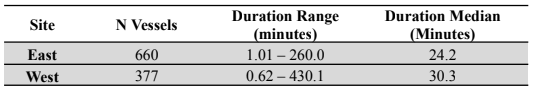
\includegraphics{images/Table.3.PNG}

\hfill\break

\begin{figure}[H]

{\centering 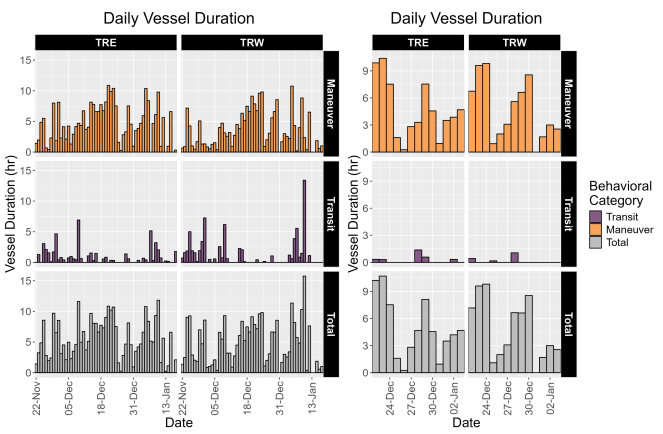
\includegraphics{images/Figure.2.PNG}

}

\caption{\textbf{Figure 2:} Daily vessel duration (hour) separated by
site. Left: Total deployment length, Right: Two-week subset of dates
highlighting vessel presence surrounding Christmas and New Year's Day
holidays. TRE = Two Rocks East; TRW = Two Rocks West.}

\end{figure}%

\section{Weekday Vessel Presence}\label{weekday-vessel-presence}

At both TRE and TRW, there was a pattern of higher vessel activity in
the latter half of the week, with the highest number of vessels
occurring on Thursdays (TRE: N = 117; TRW: N = 89). Over half of all
vessels occurred between Thursdays and Saturdays (TRE: N = 530, 80.3\%;
TRW: N = 237, 62.9\%) (Fig. 3).

Both sites showed the lowest overall activity on Mondays (TRE: N = 71,
10.7\%; TRW: N = 39, 10.3\%) and Sundays (TRE: N = 80, 12.1\%; TRW: N =
40, 10.6\%).

\begin{figure}[H]

{\centering 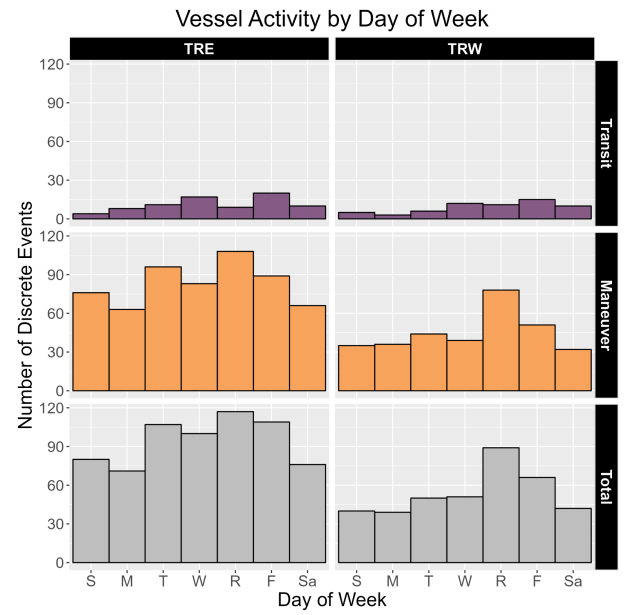
\includegraphics{images/Figure.3.PNG}

}

\caption{\textbf{Figure 3:} Vessel activity by day of week at each site.
TRE = Two Rocks East, TRW = Two Rocks West.}

\end{figure}%

\section{Diel Vessel Presence}\label{diel-vessel-presence}

Based on sunrise (05:05 -- 05:28) and sunset (19:01 -- 19:26) times
throughout the deployment, most vessels at both sites occurred during
daylight hours (05:00 -- 18:00; TRE: N = 607, 92.0\%, median = 52.5
vessels/hour; TRW: N = 329, 80.6\%, median = 28.5 vessels/hour). The
highest number of vessels in a single hour occurred at 07:00 at TRE (N =
80) and at 08:00 at TRW (N = 43) (Fig. 4).

Outside of these hours, the highest presence was in the 04:00 hour just
before sunrise (TRE: N = 26; TRW: N = 15). The remaining hours (20:00 --
03:00) were consistently lower in vessel counts (TRE: median = 2
vessels/hour, range = 0 -- 7; TRW: median = 3 vessels/hour, range = 1 -
7).

\begin{figure}[H]

{\centering 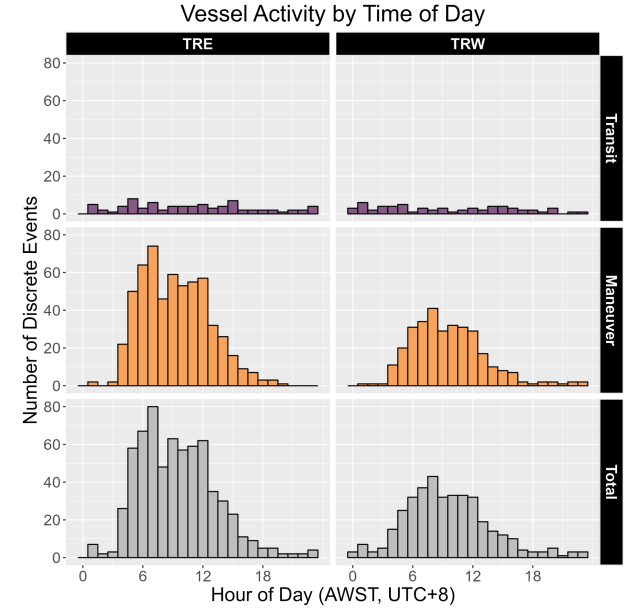
\includegraphics{images/Figure.4.PNG}

}

\caption{\textbf{Figure 4:} Counts of vessel signatures per hour at each
site. Hourly presence counts reflect the start time of each vessel
signature. Times are reported in local time (AWST, UTC +8).}

\end{figure}%

\section{Propagation modeling and detection
range}\label{propagation-modeling-and-detection-range}

The following transmission loss (TL) equation was fit using empirical RL
data from the calibration tracks made at TRE (Eq. 1, Fig. 5). The TRW
calibration tracks did not result in a plausible model of transmission
loss, but due to similarity of habitat between the two sites, the TL
model from TRE was used to determine vessels likely to occur within the
NPZ boundaries for both sites.

(Eq. 1): \[
TL_{TRE} = 19.94((r)) + 0.0000r
\]

\begin{figure}[H]

{\centering 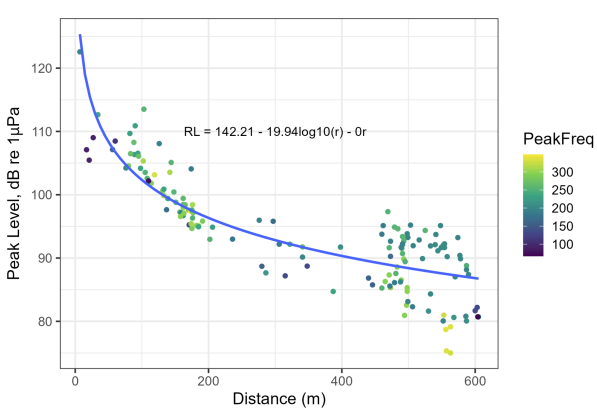
\includegraphics{images/Figure.5.PNG}

}

\caption{\textbf{Figure 5:} Regression line of received levels measured
from acoustic recordings versus deployment vessel ranges taken from GPS
points taken from Two Rocks East (TRE) sites. Color scale indicates peak
frequency value of sound for each sound clip.}

\end{figure}%

Modeled transmission loss and ambient noise levels were similar between
TRE and TRW, with \(NL_{50}\) values of 82.7 dB re 1μPa at TRE and 81.1
dB re 1μPa at TRW. The maximum detection distance for a representative
medium-sized vessel at each site was also similar between the sites: TRE
= 13.4 km, TRW = 16.1 km. The weighted mean distance between the
recorder and the park boundary was 1851 meters for TRE and 1779 meters
for TRW.

\section{Total Vessel Presence within Park
Boundaries}\label{total-vessel-presence-within-park-boundaries}

For TRE, 548 of the original 660 vessels were usable for propagation
analysis. Of those, 181 (33.0\% of usable vessels) were likely to occur
within the NPZ boundary assuming they were small vessels (SL: 125 -- 150
dB re 1μPa). Of those, 172 vessel signatures contained a maneuver
(95.0\%) (Table 4). Further, there were 33 vessels (6.0\% of usable
vessels) estimated to occur within the NPZ assuming they were either
small or medium vessels (SL: 125 -- 170 dB re 1μPa), with 31 signatures
(93.9\%) containing a maneuver (Table 4).

At TRW, 327 of the original 377 vessels were usable for propagation
analysis. There were 105 vessels (32.1\% of usable vessels) with
\(P_{small\;in} > 0.75\). Of those, a majority of the signatures
contained a maneuver (N = 100, 95.2\%). If vessels were assumed to
belong to either a small or medium size class, then 28 vessels (8.6\% of
usable vessels) were estimated to occur within the NPZ boundary. Of
these, all signatures contained a maneuver.

At both sites, vessels were present inside the park boundary
(\(P_{in} > 0.75\)) throughout the deployment, with the highest daily
vessel presence by duration occurring in late December (TRE: December
23, 1.78 hours; TRW: December 29, 2.72 hours) (Fig. 6).

\textbf{Table 4:} Summary of vessel presence and vessels at each
recording site estimated to occur within the park boundaries surrounding
Two Rocks East and Two Rocks West sites.
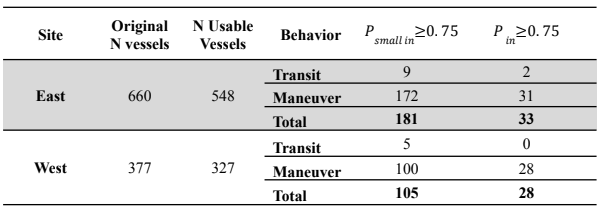
\includegraphics{images/Table.4.PNG}

\begin{figure}[H]

{\centering 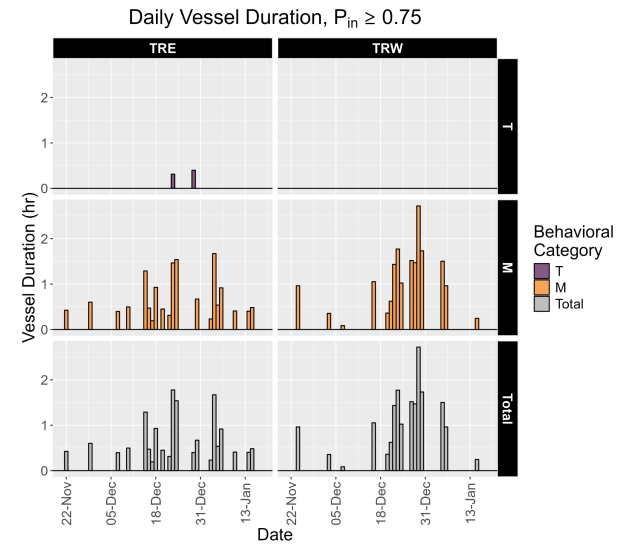
\includegraphics{images/Figure.6.PNG}

}

\caption{\textbf{Figure 6:} Daily vessel duration (hour) of vessels
estimated within park boundaries(\(P_{in} > 0.75\)) T = transit, M =
maneuver.}

\end{figure}%

\section{Weekday Vessel Presence within Park
Boundaries}\label{weekday-vessel-presence-within-park-boundaries}

At TRE, Fridays had the highest vessel presence (N = 8), followed by
Saturdays, Thursdays, and Tuesdays (N = 6 each day) (Fig. 7). The two
transiting vessels without a maneuver occurred on Thursday and Friday (N
= 1 vessel each day). At TRW, there was a more apparent effect of
weekday, with 39.3\% of all vessels with \(P_{in} > 0.75\) occurring on
Thursdays (N = 11).

\begin{figure}[H]

{\centering 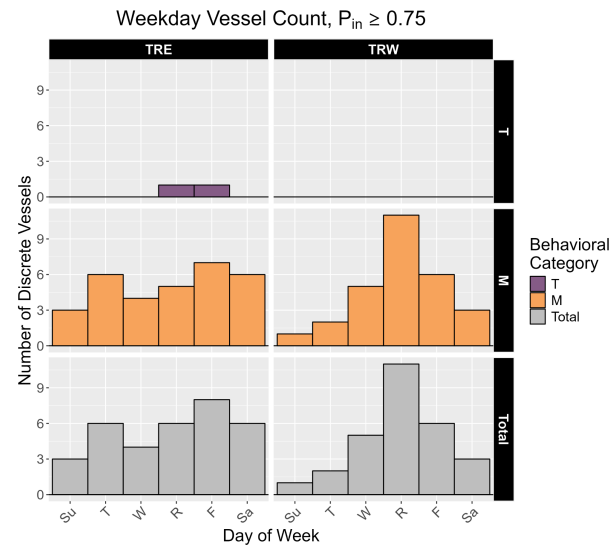
\includegraphics{images/Figure.7.PNG}

}

\caption{Figure 7: Vessel activity by day of week and behavioral
category of vessels estimated within park boundaries(\(P_{in} > 0.75\))
T = transit, M = maneuver.}

\end{figure}%

\section{Diel Vessel Presence within Park
Boundaries}\label{diel-vessel-presence-within-park-boundaries}

At TRE, all vessels with \(P_{in} > 0.75\) occurred between 00:00 -
15:00 AWST (range = 1 -- 7 per hour) (Fig. 8). The highest number of
vessels during a single hour occurred at 12:00 AWST (N = 7), with all of
those vessels containing a maneuver. Transiting vessels without a
maneuver were detected at 06:00 and 14:00 (N = 1 each hour).

TRW showed a similar concentration of vessel activity early in the day,
with the majority of vessels within the NPZ occurring between 05:00 and
15:00 AWST (N = 32, range = 1 -- 6 per hour) (Fig. 8). The single vessel
outside of daylight hours occurred at 22:00 AWST. Vessel activity peaked
at 10:00 (N = 6), with a secondary peak at 08:00 (N = 4).

\begin{figure}[H]

{\centering 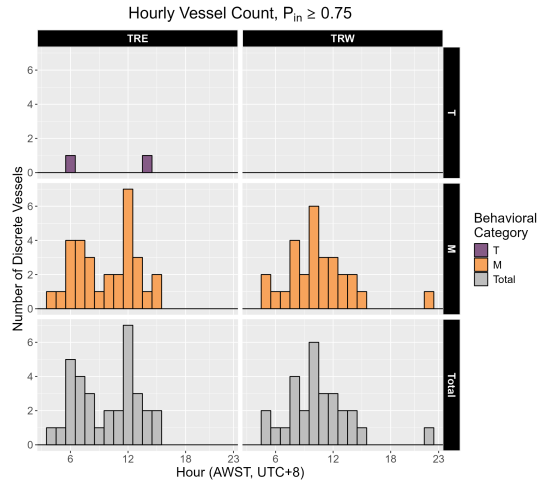
\includegraphics{images/Figure.8.PNG}

}

\caption{Figure 8: Counts of vessel signatures estimated within park
boundaries(\(P_{in} > 0.75\)) per hour separated by behavioral category.
Hourly presence counts reflect the start time of each vessel signature.
Times are reported in local time (AWST, UTC+8). T = transit, M =
maneuver.}

\end{figure}%

\bookmarksetup{startatroot}

\chapter{Discussion and
Recommendations}\label{discussion-and-recommendations}

\section{Patterns of vessel presence}\label{patterns-of-vessel-presence}

Vessel signatures were present throughout the recordings made at two
sites within the Two Rocks Marine Park NPZ. The deployment period
captured vessel presence during two major holidays: Christmas Day
(25-Dec) and New Year's Day (01-Jan). Vessels, particularly those
containing maneuvers, increased in presence leading up to each holiday;
however, the holidays themselves showed a marked decrease in presence.
Overall, vessels were most prevalent towards the end of the week, and
this general pattern may have contributed to lower presence on Christmas
Day and New Year's Day which both occurred on Sundays during the
deployment period. Total vessel presence was also highest during
daylight hours, which is consistent with other monitored parks.

The majority of vessels were estimated to occur outside of the park
boundaries (\(P_{in} > 0.75\)) = TRE: 33/548 usable vessels, 94.0\%;
TRW: 28/327 usable vessels, 91.4\%), which suggests relatively high
compliance as in other analyzed NPZs: Ningaloo Marine Park
(nwninnpz02)(McCordic et al.~2021), Dampier Marine Park (nwdamnpz01)
(McCordic et al.~2022), Cod Grounds Marine Park (tecodnpz01) (Kline et
al.~2020; McCordic et al.~2020), Solitary Islands Marine Park
(tesolnpz02) (Kline et al.~2020; McCordic et al.~2020). Vessels within
the NPZ boundaries showed similar temporal patterns in terms of weekday
and diel presence as the patterns seen in all detected vessels. Most
vessels occurred late in the week and on weekends, and most vessels were
present within the NPZ boundaries between late morning and early
afternoon. Between the two sites, the majority of vessels within the NPZ
boundaries contained maneuvers, and vessels with maneuvers were driving
the observed weekday and diel patterns of vessels within the NPZ.

\section{Recommendations for
monitoring}\label{recommendations-for-monitoring}

As seen previously at Two Rocks Marine Park, the total vessel counts
over the deployment period are considerably higher than other reported
NPZs, which is likely due to the proximity of the park to Perth as well
as its proximity to shore. Despite a low recall value of the detector at
both sites, due to the overall high vessel numbers in Two Rocks Marine
Park and a relatively high precision of the detector, the ship detector
alone is likely sufficient to determine general patterns of vessel
presence without additional manual review.

Vessels were estimated to occur within the NPZ boundaries throughout the
entire deployment period, and the majority of those vessels contained at
least one maneuver. Although a maneuver is not diagnostic of a vessel's
specific activity, it can be used as a proxy for fishing activity and
warrants further investigation (e.g., Kline et al.~2020). Similar to
total vessel presence, activity of vessels estimated within the NPZ
boundaries showed a peak prior to the Christmas and New Year's Day
holidays.

Due to the high prevalence of vessel signatures late in the
week---Thursday through Saturday---we recommend increased patrol efforts
on these days. During holiday periods, additional surveys on days
leading up to holidays may also result in increased interactions with
vessels in the NPZ rather than surveying on the holidays themselves.
This pattern may change in other years, however, depending on the
weekday on which holidays occur (e.g., if the holidays fall on a later
weekday rather than a Sunday). Since the majority of vessels occur early
in the day, visual patrols (aerial or ship-based) focusing on these
times would provide a valuable complement to the results presented here.

\bookmarksetup{startatroot}

\chapter*{References}\label{references}
\addcontentsline{toc}{chapter}{References}

\markboth{References}{References}

\printbibliography[heading=none]


\backmatter


\end{document}
